\documentclass[a4paper,12pt]{article}

% Основные пакеты
\usepackage[T1, T2A]{fontenc}
\usepackage[utf8]{inputenc}
\usepackage[english, russian]{babel}
\usepackage{geometry}
\usepackage{indentfirst}
\usepackage{graphicx}
\usepackage{wrapfig}
\usepackage{amsmath, amssymb, amsfonts}
\usepackage{braket} 
\usepackage{float}
\usepackage{bm}  

% Гиперссылки и цветовые настройки
\usepackage[dvipsnames]{xcolor}
\usepackage[colorlinks]{hyperref}
\hypersetup{
	linkcolor=blue,
	filecolor=magenta,
	urlcolor=cyan
}

\usepackage{listings}

% Стиль для Bash листингов
\definecolor{shellbg}{RGB}{240,240,240}
\definecolor{shellprompt}{RGB}{64,128,64}
\definecolor{shellcommand}{RGB}{0,0,0}
\definecolor{shelloutput}{RGB}{128,0,0}


% Цвета для общего стиля листингов
\definecolor{backcolour}{rgb}{0.95,0.95,0.92}
\definecolor{codegreen}{rgb}{0, 0.5, 0}
\definecolor{codegray}{rgb}{0.4, 0.4, 0.4}
\definecolor{codepurple}{rgb}{0.58, 0, 0.82}
\definecolor{keywordcolor}{rgb}{0.0, 0.2, 0.7}
\definecolor{stringcolor}{rgb}{0.6, 0, 0}
\definecolor{framecolor}{rgb}{0.7, 0.7, 0.7}

% Стиль для листингов с поддержкой русского языка
\lstdefinestyle{russian}{
	backgroundcolor=\color{backcolour},
	basicstyle=\ttfamily\small,
	keywordstyle=\color{keywordcolor}\bfseries,
	commentstyle=\color{codegreen}\itshape,
	stringstyle=\color{stringcolor},
	numberstyle=\tiny\color{codegray},
	numbers=left,
	numbersep=5pt,
	breaklines=true,
	breakatwhitespace=false,
	showstringspaces=false,
	keepspaces=true,
	frame=single,
	rulecolor=\color{framecolor},
	frameround=tttt,
	captionpos=b,
	tabsize=2,
	xleftmargin=1em,
	xrightmargin=0.1em,
	literate=
	{а}{{\selectfont\char224}}1
	{б}{{\selectfont\char225}}1
	{в}{{\selectfont\char226}}1
	{г}{{\selectfont\char227}}1
	{д}{{\selectfont\char228}}1
	{е}{{\selectfont\char229}}1
	{ё}{{\"e}}1
	{ж}{{\selectfont\char230}}1
	{з}{{\selectfont\char231}}1
	{и}{{\selectfont\char232}}1
	{й}{{\selectfont\char233}}1
	{к}{{\selectfont\char234}}1
	{л}{{\selectfont\char235}}1
	{м}{{\selectfont\char236}}1
	{н}{{\selectfont\char237}}1
	{о}{{\selectfont\char238}}1
	{п}{{\selectfont\char239}}1
	{р}{{\selectfont\char240}}1
	{с}{{\selectfont\char241}}1
	{т}{{\selectfont\char242}}1
	{у}{{\selectfont\char243}}1
	{ф}{{\selectfont\char244}}1
	{х}{{\selectfont\char245}}1
	{ц}{{\selectfont\char246}}1
	{ч}{{\selectfont\char247}}1
	{ш}{{\selectfont\char248}}1
	{щ}{{\selectfont\char249}}1
	{ъ}{{\selectfont\char250}}1
	{ы}{{\selectfont\char251}}1
	{ь}{{\selectfont\char252}}1
	{э}{{\selectfont\char253}}1
	{ю}{{\selectfont\char254}}1
	{я}{{\selectfont\char255}}1
	{А}{{\selectfont\char192}}1
	{Б}{{\selectfont\char193}}1
	{В}{{\selectfont\char194}}1
	{Г}{{\selectfont\char195}}1
	{Д}{{\selectfont\char196}}1
	{Е}{{\selectfont\char197}}1
	{Ё}{{\"E}}1
	{Ж}{{\selectfont\char198}}1
	{З}{{\selectfont\char199}}1
	{И}{{\selectfont\char200}}1
	{Й}{{\selectfont\char201}}1
	{К}{{\selectfont\char202}}1
	{Л}{{\selectfont\char203}}1
	{М}{{\selectfont\char204}}1
	{Н}{{\selectfont\char205}}1
	{О}{{\selectfont\char206}}1
	{П}{{\selectfont\char207}}1
	{Р}{{\selectfont\char208}}1
	{С}{{\selectfont\char209}}1
	{Т}{{\selectfont\char210}}1
	{У}{{\selectfont\char211}}1
	{Ф}{{\selectfont\char212}}1
	{Х}{{\selectfont\char213}}1
	{Ц}{{\selectfont\char214}}1
	{Ч}{{\selectfont\char215}}1
	{Ш}{{\selectfont\char216}}1
	{Щ}{{\selectfont\char217}}1
	{Ъ}{{\selectfont\char218}}1
	{Ы}{{\selectfont\char219}}1
	{Ь}{{\selectfont\char220}}1
	{Э}{{\selectfont\char221}}1
	{Ю}{{\selectfont\char222}}1
	{Я}{{\selectfont\char223}}1
}



% Установить стиль по умолчанию
\lstset{style=russian}

% Геометрия страницы
\geometry{left=2cm, right=2cm, bottom=2cm, top=2cm}

\begin{document}
	\begin{titlepage}
		\centering
		\vspace*{1cm}
		
		{\large Министерство науки и высшего образования Российской Федерации}\\
		{\large ФЕДЕРАЛЬНОЕ ГОСУДАРСТВЕННОЕ АВТОНОМНОЕ ОБРАЗОВАТЕЛЬНОЕ УЧРЕЖДЕНИЕ ВЫСШЕГО ОБРАЗОВАНИЯ «НАЦИОНАЛЬНЫЙ ИССЛЕДОВАТЕЛЬСКИЙ УНИВЕРСИТЕТ ИТМО»}\\
		{\large (УНИВЕРСИТЕТ ИТМО)}\\
		
		\vspace{2cm}
		
		{\large Факультет «Систем управления и робототехники»}\\
		
		\vspace{3cm}
		
		\textbf{{\Huge ОТЧЕТ}\\
			{\Huge О ЛАБОРАТОРНОЙ РАБОТЕ №0}}\\
		
		\vspace{1cm}
		
		{\LARGE По дисциплине «Машинное обучение»}\\
		{\LARGE на тему: «Знакомство с системой контроля версий git и сервисом GitHub»}\\
		
		\vspace{3cm}
		
		{\Large Студент:}\\
		Охрименко Е. Д. 
		
		\vspace{2cm}
		
		{\Large Преподаватели:}\\
		Усачева Д. М.\\
		Поляк М. Д.\\
		
		\vspace{3cm}
		{\large г. Санкт-Петербург}\\
		{\large 2025}
		
	\end{titlepage}
	\newpage
	
	
	\section{Задание 1.}
	\textbf{Цель: }  поразмышлять о своих целях и задачах на текущий семестр.
	
	\begin{itemize}
		\item С помощью веб-интерфейса GitHub создать файл \texttt{goals.md} в своем репозитории.
		\item Используя язык разметки markdown, создать заголовки <<Мой опыт>> и <<Мои цели>>.
		\item Написать один абзац (1-5 предложений) о своем опыте по разработке программного обеспечения. Добавить работающую ссылку в написанный текст (например, на ваш профиль в \texttt{GitHub}).
		\item Создать нумерованный список из 2 или 3 целей, которых планируете достичь в рамках данного курса.
		\item Создать ненумерованный список из 3-9 задач, над которыми собираетесь работать в рамках данного курса для достижения поставленных целей.
		\item Создать папку \texttt{resources} в корне репозитория. Загрузить в эту папку изображение (\texttt{.png/.jpg/.jpeg}) и добавить его в ваш \texttt{.md} файл.
		\item Закоммитить файлы в свой репозиторий на \texttt{GitHub}.
		\item Проверить, что созданный \texttt{.md} файл отформатирован и отображается при предпросмотре именно так, как планировалось.
	\end{itemize}
	
	Я создала в корне репозитория файл goals.md и, используя язык разметки markdown, написала пару абзацев и вставила картинку, предварительно загруженную в папку resources.\\
	
	\begin{lstlisting}[caption={Содержимое файла \texttt{goals.md}}]
## Мой опыт
> У меня есть небольшой опыт в разработке ПО, я строила карту по лидару, и, используя **SLAM**, пыталась научить робота объезжать препядствие. Это занятие мне не очень понравилось, поэтому я на данный момент изучаю **Java** и имею желание и дальше развиваться в сфере программирования. Ссылка на мой профиль: [GitHub](https://github.com/decadeos/).
## Мои цели
> В рамках курса мне бы хотелось:
1. Сформировать понимание алгоритмов **ML**.
2. Научиться пользваться основными библиотеками **python**, которые нужны для анализа данных.
3. Реализовать как минимум одну работающую модель обучения, решающую практическую задачу.

> Чтобы достичь поставленных целей мне нужно:
- [ ] Стараться посещать все лекции и практические занятия.
- [ ] Читать дополнительную литерауру.
- [x] Быть заинтересованной в получении новых знаний.
- [ ] При написании кода понимать буквально все, что написано, вплоть до мелочей.

![ ](https://github.com/decadeos/ml-lab0-decadeos/blob/main/resources/capibara.png)
\end{lstlisting}
	
\begin{figure}[H]
	\centering
	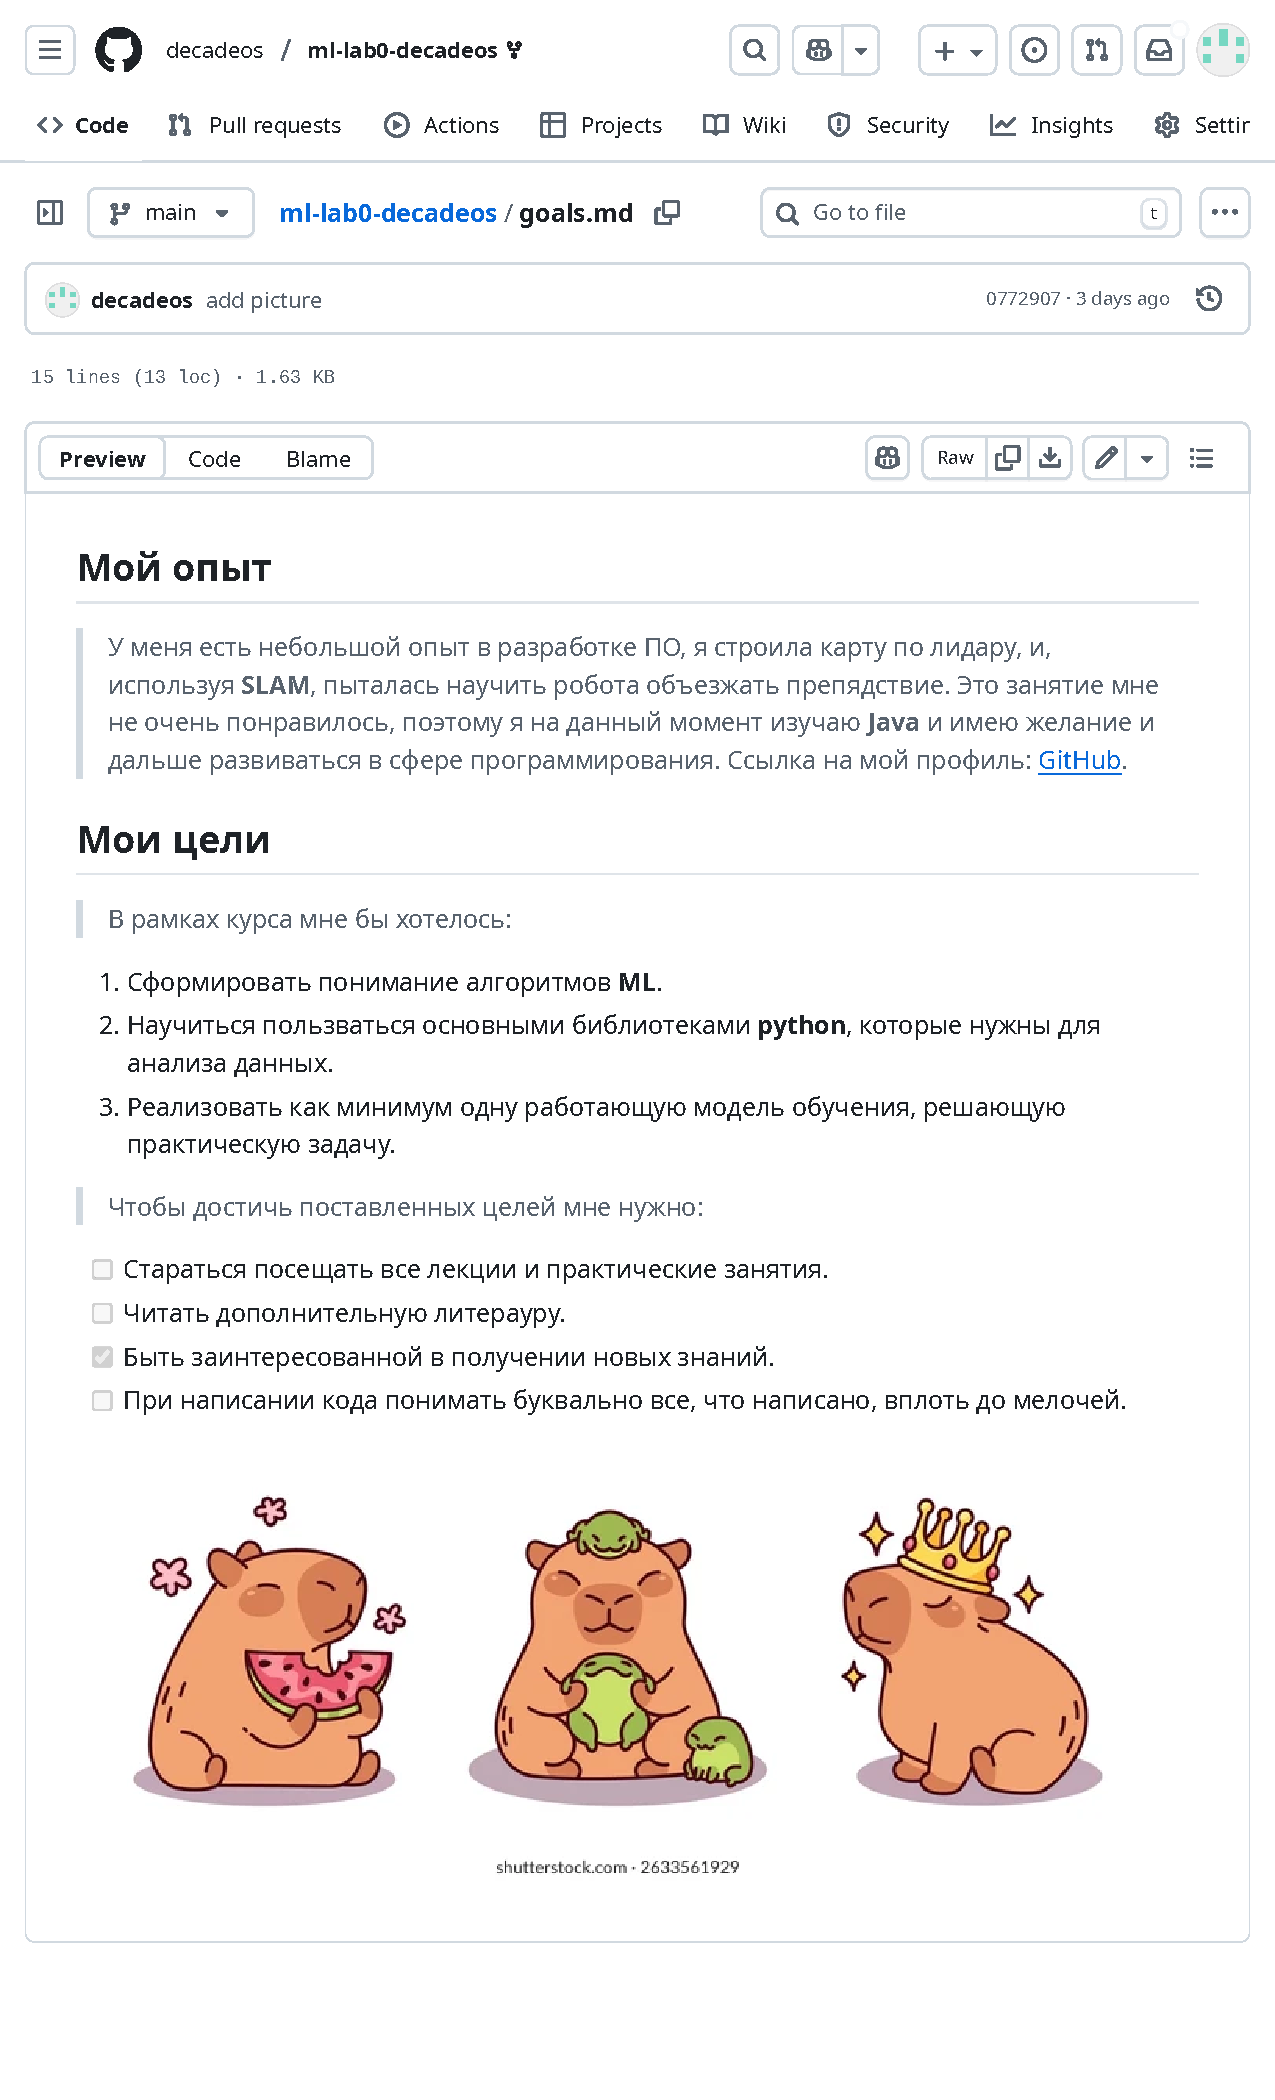
\includegraphics[width=0.88\textwidth]{../resources/goals.pdf}
	\caption{Отображение файла \texttt{goals.md}}
\end{figure}
	
	\newpage


\section{Задание 2.}

\textbf{Цель: } научиться использовать git из командной строки.
	
	
\begin{itemize}
	\item Ознакомьтесь с инструкцией по работе с git и github из командной строки.
	\item Клонируйте свой репозиторий на локальный компьютер используя команду \texttt{git clone <ссылка на ваш репозиторий>} из командной строки.
	\item Создайте новый файл \texttt{info.md} в своей локальной копии репозитория.
	\item Запишите в этот файл свое ФИО (полностью), название используемой операционной системы, текущие дату и время - каждый элемент с новой строки (всего получится 3 строки).
	\item Выполните команды \texttt{git add info.md} и \texttt{git commit} в командной строке.
	\item Введите краткое описание коммита.
	\item Выполните команду \texttt{git push}.
	\item Создайте папку \texttt{data} в корне репозитория и в ней файл \texttt{dataset.csv}.
	\item Создайте файл \texttt{.gitignore}, в который добавьте строку \texttt{data/}.
	\item Закоммитьте \texttt{.gitignore} и попробуйте закоммитить \texttt{data/dataset.csv}, после чего отправьте коммиты в репозиторий на github.com с помощью \texttt{git push}.
	\item Объясните полученный результат в отчёте.
\end{itemize}

Я склонировала себе репозиторий, заполнила файл \texttt{info.md}. 

\begin{lstlisting}[caption={Содержимое файла \texttt{info.md}}]
Охрименко Ева Дмитриевна

Ubuntu 20.04.6 LTS

2025.09.16 22:01
\end{lstlisting}

Я поставила переносы строк между строчками, так как без них в репозитории на \texttt{GitHub} все три строки сливаются в один сплошной текст.

\begin{figure}[H]
	\centering
	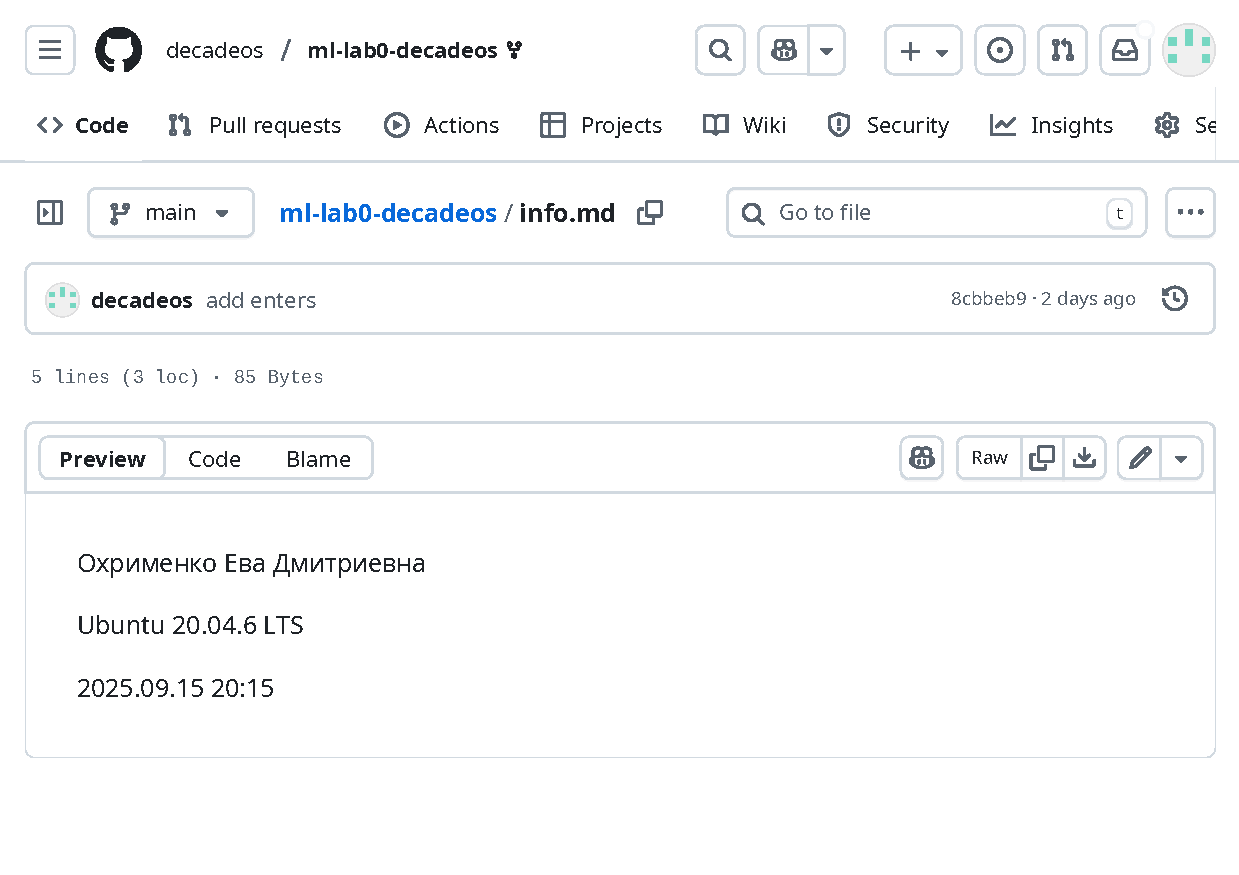
\includegraphics[width=1\textwidth]{../resources/info.pdf}
	\caption{Отображение файла \texttt{info.md}}
\end{figure}

Далее я создала директорию \texttt{data/} и в ней создала файл \texttt{dataset}. Закоммитила изменения.

Затем в корне репозитория я создала файл \texttt{.gitignore} и записала туда строчку \texttt{data/}. 

\begin{lstlisting}[caption={Содержимое файла \texttt{.gitignore}}]
data/

/latex/*
!/latex/*.tex
!/latex/*.pdf
\end{lstlisting}

Это означает, что  мне не удасться ни проиндексировать папку, ни закоммитить ее. Также в \texttt{.gitignore} я добавлю временные LaTeX-файлы.

\begin{lstlisting}[caption={Попытка индексации \texttt{data/}}]
eva@eva:~/Documents/ML/ml-lab0-decadeos$ git add data/ 
The following paths are ignored by one of your .gitignore files:
data
Use -f if you really want to add them.
\end{lstlisting}

\texttt{git} сообщает, что папка \texttt{data/} игнорируется и не может быть проиндексирована. Если очень хочется, можно использовать флаг \texttt{---force} и принудительно добавить ее в коммит.

\end{document}

